\documentclass{article}
	\title{A Practical Attack to De-Anonymize Social Network Users - Summary}
	\author{Sandeep Reddy Salla}
	\usepackage{graphicx}
	\graphicspath{{D:/Marist Spring 2016/Security Algo/HistoryStealing/}}
	
\begin{document}
\maketitle

De-anonymization attack can be performed on group members of a group on social networking sites like Facebook, twitter, Xing, etc. (they have similar structure) to get the information of group members or about specific users. De-anonymization attack is practically done on Xing social network. The results indicate 42\% of users present in this network that use groups can be affected.\\
\begin{enumerate}
\item Two types of \textbf{groups} on social network:
	\begin{itemize}
	\item 	\textbf{Public Group:}  Any member of the social network can join into this group. Authorization is not required.
	\item \textbf{Closed Group:} It requires some authorization before joining into this group.
	\end{itemize}


\item \textbf{History stealing} is one of the main techniques an attacker can use. With the help of this technique attacker can keep track of the victim’s browser history for certain URLs which will reveal the group members on a social network.\\

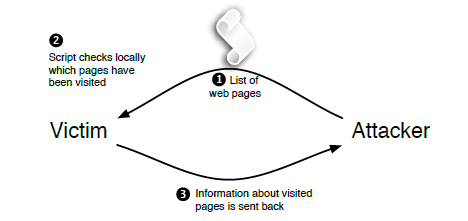
\includegraphics{HistoryStealing.png}

\item \textbf{Model and Definition:}
Social Networks \emph{S} is represented as a graph G.
	\begin{equation}
		G = (V,E)
	\end{equation}
where \emph{V} represents users and \emph{E} represents friendship between users.\\
	\\$\Gamma (\emph{v}) := (\Gamma g(\emph{v}))_ {g\epsilon G}$	
\\$\Gamma g(\emph{v})=1$
If \emph{v} is a member of group \emph{g}

$\Gamma g(\emph{v})=0$
If \emph{v} is not a member of group \emph{g}


\item\textbf{Efficiently Obtaining Group Information:}
\begin{itemize}
	\item \textbf{Group Directory:} Group directory can be reconstructed if attacker guesses the group IDs.
	\item \textbf{Group Member Crawling:} To gain information about members of the group, attacker also needs to keep track of the ID’s of the members of the group along with the group IDs.
\end{itemize}


\item\textbf{Social Network Crawling Approaches:}
\begin{itemize}
	\item \textbf{Customer Crawler:} Web crawler has been implemented to follow the hyperlinks of a public page to download HTML source code in order to access the parts of social network (restricted to members).
	\item \textbf{Commercial Crawling Service:} Attackers with less number of network resources lead to commercial crawling service.
\end{itemize}

\item\textbf{Crawling Experiment Results:}
\begin{itemize}
	\item \textbf{Xing:} Automated member requests are sent to 1306 closed groups, 108 groups accepted. This allowed an attacker to track the user IDs of total groups.	
	\item \textbf{Facebook:} Using two machines, 43.2 million members of the group are crawled from 31,853 groups in a span of 23 days.
	\item \textbf{LinkedIn:} Two phase crawling scenario has been implemented. In the first scenario, collected 3 million hyperlinks from the observed group Ids space. In the second phase, additional information like group size, description has been retrieved.
\end{itemize}


\item\textbf{Mitigation Techniques:}
\begin{itemize}
	\item \textbf{Server-side Mitigation:} To send parameter values in an URL, web application must use HTTP POST instead of HTTP GET.
	\item \textbf{Client-side Mitigation:} Restrict the properties of cascading style sheet of hyperlinks, disable browsing history.
\end{itemize}
\end{enumerate}

\end{document}